
%dash pattern=on 5pt off 2pt
%[fill = white, rounded corners = 5pt, inner sep=0.8pt]
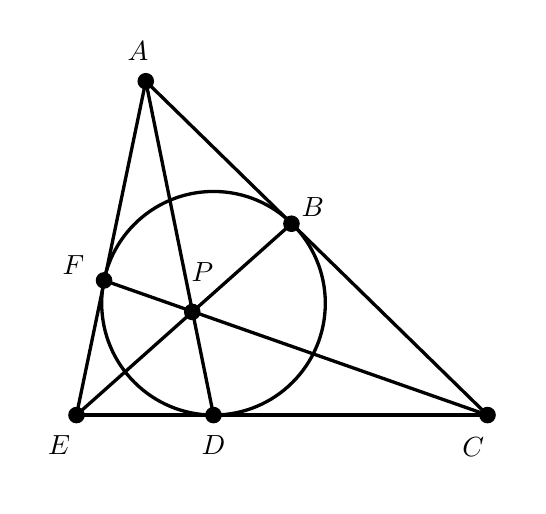
\begin{tikzpicture}[scale = 1]
    \clip(-2.26,-0.34) rectangle (3.96,5.48);
    \draw [line width=1.2pt] (-0.76,4.8)-- (-1.64,0.56);
    \draw [line width=1.2pt] (-1.64,0.56)-- (3.58,0.56);
    \draw [line width=1.2pt] (3.58,0.56)-- (-0.76,4.8);
    \draw [line width=1.2pt] (0.1,1.98) circle (1.42cm);
    \draw [line width=1.2pt] (-0.76,4.8)-- (0.1,0.56);
    \draw [line width=1.2pt] (-1.64,0.56)-- (1.09,2.99);
    \draw [line width=1.2pt] (3.58,0.56)-- (-1.29,2.27);
    \begin{scriptsize}
        \normalsize
        \fill [color=black] (-0.76,4.8) circle (3.0pt);
        \draw[color=black] (-0.86,5.18) node {$A$};
        \fill [color=black] (-1.64,0.56) circle (3.0pt);
        \draw[color=black] (-1.86,0.18) node {$E$};
        \fill [color=black] (3.58,0.56) circle (3.0pt);
        \draw[color=black] (3.4,0.16) node {$C$};
        \fill [color=black] (1.09,2.99) circle (3.0pt);
        \draw[color=black] (1.36,3.2) node {$B$};
        \fill [color=black] (0.1,0.56) circle (3.0pt);
        \draw[color=black] (0.1,0.18) node {$D$};
        \fill [color=black] (-1.29,2.27) circle (3.0pt);
        \draw[color=black] (-1.68,2.46) node {$F$};
        \fill [color=black] (-0.17,1.87) circle (3.0pt);
        \draw[color=black] (-0.04,2.38) node {$P$};
    \end{scriptsize}
\end{tikzpicture}